\chapter{Probabilistic Modeling}

\section{Modeling with Probability Distributions}

% use this section to illustrate modeling with a poisson rv
At a facility that manufactures recreational sports
  vehicles (ATVs), each vehicle is subjected to a final
  inspection. The rate of defects during final inspection is
  $\lambda=1.5$ defects per vehicle.
\begin{enumerate}
\item What is an appropriate probability distribution to model the
number of defects? \label{atv1}
\item What proportion of vehicles have more than 2 defects? \label{atv2}
\item Management has set a new goal that the proportion
of vehicles with no defects is .5. What rate $\lambda$ would
achieve this goal? \label{atv3}
\end{enumerate}

We are interested in the number of defects, which is discrete.
The Poisson distribution makes sense because it is commonly used
for count data. Moreover, we are given information for a single
parameter, and the Poisson distribution has a single parameter.
If we let the random variable $X$ represent the number of defects
per vehicle, then a reasonable distribution is
\[ X \sim \text{Poisson}(\lambda=1.5) \]
For part~\ref{atv2},
\begin{align*}
P(X>2) &= 1 - P(X \leq 2)\\
       &= 1 - \sum_{x=0}^2 \frac{e^{-\lambda}\lambda^x}{x!}\\
       &= 0.191
\end{align*}
For part \ref{atv3}, management's goal is that $P(X=0)=0.5$, or
\[ P(X=0) = \frac{e^{-\lambda}\lambda^0}{0!} = e^{-\lambda}=0.5 \]
Then
\[ \lambda = -\ln{0.5} = 0.693 \]

\section{Stochastic Processes}

% Use this section to introduce the idea of a Poisson Process.
% add explanatory material.
\emph{A Poisson Process.} A statistician has observed the behavior of a Hollywood celebrity for
about one year and has noted that between the hours of 8pm and 11pm
this celebrity generates, on average, three tweets per hour and that
the rate is approximately the same within each one-hour period.  We
can count the \emph{number} of tweets that occur in a time interval
$t$. We can also measure the \emph{time} between tweets. Here is a
depiction of the tweets from last night.

\vspace{.2in}
\begin{center}
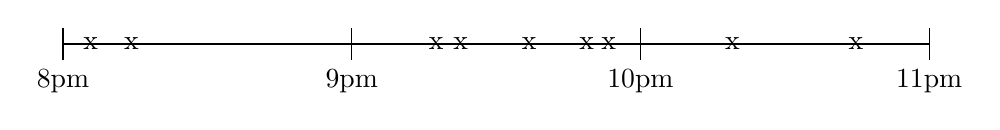
\begin{tikzpicture}

\draw (0,0) -- (11,0)
  node[pos=0.35/11]{x}
  node[pos=0.87/11]{x}
  node[pos=4.74/11]{x}
  node[pos=5.05/11]{x}
  node[pos=5.92/11]{x}
  node[pos=6.65/11]{x}
  node[pos=6.93/11]{x}
  node[pos=8.50/11]{x}
  node[pos=10.07/11]{x}
;
\node[below] at (0,-.2) {8pm};
\draw (0,-.2) -- (0,.2);
\node[below] at (11/3,-.2) {9pm};
\draw (11/3,-.2) -- (11/3,.2);
\node[below] at (22/3,-.2) {10pm};
\draw (22/3,-.2) -- (22/3,.2);
\node[below] at (11,-.2) {11pm};
\draw (11,-.2) -- (11,.2);


\end{tikzpicture}
\end{center}

Let the random variable $Y$ be the number of tweets from
the celebrity in some time interval.
When we say that the number of tweets in a time interval $t$ follows
a Poisson distribution with mean $\lambda t$, we write
\[
  Y \sim \text{Poisson($\lambda t$)}
\]
If $t$ is one hour, then we can write
\[
  Y \sim \text{Poisson($\lambda = 3$)}
\]
Stating that the number of tweets follows a Poisson distribution
implies that the time between tweets follows an Exponential
distribution (and vice versa). Let the random variable $X$ be
the time between tweets. Then
\[
  Y \sim \text{Poisson($\lambda t$)} \Longleftrightarrow X \sim \text{Exp($\lambda$)}
\]
Yes, it is the same $\lambda$ in each distribution.
The average number of tweets is $\lambda=3$ per hour. The average
time between tweets is $1/\lambda = 1/3$ hour (or 20 minutes).
Recall that for the Exponential distribution
\[
  E(X) = \frac{1}{\lambda} = \frac{1~\text{hour}}{3~\text{tweets}} = 20 ~\text{minutes per tweet on average}
\]

Questions.
\begin{enumerate}
  \item What is the probability that the celebrity sends out five
  or more tweets in one hour?
\item What is the probability that the celebrity sends out
  no tweets between 9pm and 11pm?
\end{enumerate}


\section{Queueing Models}

\section{Exercises}
